\section{Non-ideal Buck converter: from the circuit to the switched replica}\label{sec:model}

\subsection{Circuit and conventions}
Fig.~\ref{fig:topology} shows the asynchronous converter. The state is
$x=[i_L\;v_C]^\top$; $i_L$ flows from the switching node to the output, $i_C$
flows downward in the capacitor branch and the load disturbance $i_p$ is positive
when it draws additional current. The source is fixed, $V_{in}=\SI{48}{V}$. The
high-side switch is an IRF540N represented by its static on-resistance $R_{on}$;
the freewheel diode follows the affine conduction law of the STPST10H100SF data
sheet, $v_D=V_f+r_d i_D$ \citep{Infineon2026,ST2023}. Table~\ref{tab:params}
lists the values, all decoded from the workspace of the reference Simulink model.

\begin{figure}[t]
\centering
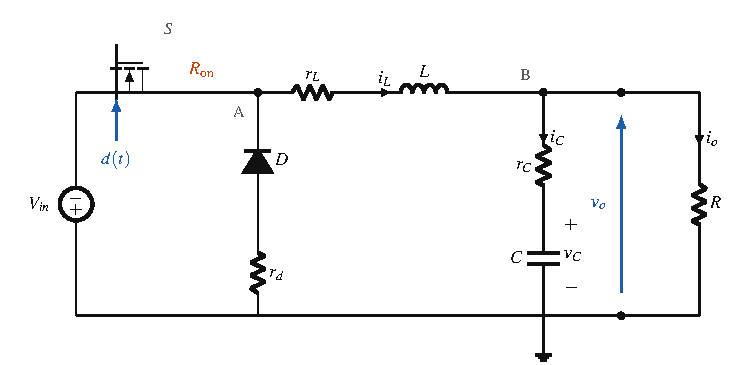
\includegraphics[width=\columnwidth]{figures/fig1_topology.pdf}
\caption{Non-ideal asynchronous Buck converter and adopted conventions.}
\label{fig:topology}
\end{figure}

\begin{table}[t]
\centering
\caption{Electrical and numerical parameters (reference model workspace).}
\label{tab:params}
\footnotesize
\begin{tabular}{@{}lll@{}}
\toprule
Quantity & Value & Role\\
\midrule
$V_{in}$ & \SI{48}{V}, constant & source\\
$L$, $r_L$ & \SI{100}{\micro H}, \SI{0.10}{\ohm} & inductor branch\\
$C$, $r_C$ & \SI{100}{\micro F}, \SI{0.05}{\ohm} & capacitor branch\\
$R$ & \SI{10}{\ohm} & nominal load\\
$R_{on}$ & \SI{0.05}{\ohm} & IRF540N static surrogate\\
$V_f$, $r_d$ & \SI{0.42}{V}, \SI{0.020}{\ohm} & STPST10H100SF affine law\\
$R_s$ ($C_s=\infty$) & \SI{100}{k\ohm} & resistive snubber across the switch\\
$R_{d,body}$ & \SI{0.01}{\ohm} & MOSFET body diode\\
$f_s$ & \SI{50}{kHz} & PWM carrier\\
$T_s$ & \SI{10}{\micro s} & controller sampling ($=1/(2f_s)$)\\
$[d_{\min},d_{\max}]$ & $[0.02,\,0.98]$ & total duty saturation\\
\bottomrule
\end{tabular}
\end{table}

\subsection{Averaged model and loss-aware equilibrium}
The output node and the ESR give
\begin{equation}
i_L=i_C+\frac{v_o}{R}+i_p,\qquad v_o=v_C+r_Ci_C,
\label{eq:node}
\end{equation}
hence
\begin{equation}
i_C=\frac{R(i_L-i_p)-v_C}{R+r_C},\qquad
v_o=\frac{R}{R+r_C}v_C+\frac{Rr_C}{R+r_C}(i_L-i_p).
\label{eq:vo}
\end{equation}
With the switch on, $L\dot i_L=V_{in}-(r_L+R_{on})i_L-v_o$; with the diode
conducting, $L\dot i_L=-V_f-(r_L+r_d)i_L-v_o$; in both cases $C\dot v_C=i_C$.
Duty averaging yields
\begin{equation}
L\dot i_L=dV_{in}-\big[r_L+dR_{on}+(1-d)r_d\big]i_L-(1-d)V_f-v_o .
\label{eq:avg}
\end{equation}
At equilibrium $I_L=V_o/R+I_p$ and the loss-aware duty is
\begin{equation}
d_{ff}=\frac{V_o+(r_L+r_d)I_L+V_f}{V_{in}-(R_{on}-r_d)I_L+V_f}.
\label{eq:dff}
\end{equation}
Every controller of this paper uses \eqref{eq:dff} with nominal parameters and
$I_p=0$ as feedforward; the feedforward never sees the simulated plant.

\subsection{Small-signal model and transfer functions}
Let $\gamma=R/(R+r_C)$, $\rho_0=r_L+r_d+d_0(R_{on}-r_d)$ and
$E_d=V_{in}+V_f-(R_{on}-r_d)I_{L,0}$. Linearizing \eqref{eq:vo}--\eqref{eq:avg}
gives $\delta\dot x=A\delta x+B_d\delta d+B_p\delta i_p$,
$\delta v_o=C_y\delta x+D_p\delta i_p$ with
\begin{equation}
A=\begin{bmatrix}-(\rho_0+\gamma r_C)/L & -\gamma/L\\ \gamma/C & -\gamma/(RC)\end{bmatrix},\;
B_d=\begin{bmatrix}E_d/L\\0\end{bmatrix},\;
C_y=\begin{bmatrix}\gamma r_C & \gamma\end{bmatrix},
\label{eq:ss}
\end{equation}
$B_p=[\gamma r_C/L\;\;-\gamma/C]^\top$ and $D_p=-\gamma r_C$. The control-to-output
transfer function is
\begin{equation}
\begin{aligned}
G_{vd}(s)&=\frac{E_dR(1+r_CCs)}{\Delta(s)},\\
\Delta(s)&=LC(R+r_C)s^2+\big[L+C\big((R+r_C)\rho_0+Rr_C\big)\big]s+R+\rho_0 ,
\end{aligned}
\label{eq:gvd}
\end{equation}
with the ESR zero $\omega_{z}=N_C=1/(r_CC)=\SI{2e5}{rad/s}$. Table~\ref{tab:tf}
instantiates \eqref{eq:dff}--\eqref{eq:gvd} at the three commanded levels; the
closed form and a state-space conversion agree to machine precision. At the
\SI{24}{V} synthesis point, $(A,B_d)$ and $(A,C_y)$ have rank two and the
integral-augmented pair has rank three.

\begin{table*}[t]
\centering
\caption{Equilibria, monic $\Delta(s)$, $G_{vd}$ numerator and stationary conduction screen at the three commanded levels (nominal load, $i_p=0$). $\omega_z=1/(r_CC)=\SI{2e5}{rad/s}$ at every level.}
\label{tab:tf}
\footnotesize
\resizebox{\textwidth}{!}{%
\begin{tabular}{@{}rrrrrllrrrr@{}}
\toprule
$V_o$ (V) & $I_{L,0}$ (A) & $d_0$ & $\rho_0$ ($\Omega$) & $E_d$ (V) & $\Delta(s)/(LC(R+r_C))$ & $G_{vd}$ numerator & $\Delta I_{L,pp}$ (A) & $I_{crit}$ (A) & $\bar I_L-I_{crit}$ (A) & $R_{crit}/R$\\
\midrule
1 & 0.1 & 0.029576 & 0.120887 & 48.417 & $s^2+2701.41s+1.00705\times10^{8}$ & $2.40881\times10^{4}s+4.81761\times10^{9}$ & 0.1941 & 0.0970 & 0.0030 & 1.030\\
24 & 2.4 & 0.511045 & 0.135331 & 48.348 & $s^2+2845.85s+1.00849\times10^{8}$ & $2.40537\times10^{4}s+4.81075\times10^{9}$ & 2.3470 & 1.1735 & 1.2265 & 2.045\\
46 & 4.6 & 0.972868 & 0.149186 & 48.282 & $s^2+2984.40s+1.00987\times10^{8}$ & $2.40209\times10^{4}s+4.80418\times10^{9}$ & 0.2496 & 0.1248 & 4.4752 & 36.856\\
\bottomrule
\end{tabular}}
\end{table*}


\subsection{Conduction mode across the range}
For a duty $d_{ff}$ the inductor ripple, the boundary current and the boundary
load are
\begin{equation}
\Delta I_{L,pp}=\frac{V_o(1-d_{ff})}{Lf_s},\qquad I_{crit}=\frac{\Delta I_{L,pp}}{2},\qquad
R_{crit}=\frac{2Lf_s}{1-d_{ff}} .
\label{eq:ccm}
\end{equation}
The stationary screen (Table~\ref{tab:tf}) is positive at every level but not
uniform: at \SI{1}{V} the current margin is \CCMmargin{} and $R_{crit}$ is only
\CCMratio{} times the nominal load. The switched model is more pessimistic than
this screen: over the steady \SI{1}{V} window it spends \DCMone{} of the time in
discontinuous conduction at \ETAone{} efficiency, because the diode drop is
\SI{42}{\percent} of the commanded output. Discontinuous conduction is thus a
nominal regime of the mission, and every controller is validated in it.

\subsection{Switched replica of the reference model}\label{sec:replica}
The acceptance model (Fig.~\ref{fig:slx}) is the Simulink/Simscape Electrical
model \texttt{buck\_fo\_lqi\_fixed\_reference\_v6\_1\_46V\_R2022a.slx}. For the
campaign we use a replica written from its block parameters
(\texttt{cmo/sim.py}): a resistive switch with snubber $R_s$ and a body diode
$R_{d,body}$; the affine freewheel diode, which blocks reverse current so that
discontinuous conduction arises by itself (the \SI{1}{ns} snubber-leakage
branch is solved quasi-statically); a continuous sawtooth carrier whose edges
are located exactly inside the integration step; a controller sampled at $T_s$
with a one-sample output delay, exactly as the S-function of the reference
model. The step is \SI{0.2}{\micro s} (100 steps per switching period) with
fourth-order Runge--Kutta integration.

The energy boundary is the one declared in the model workspace:
\begin{equation}
\begin{aligned}
P_{in}&=V_{in}i_{in},\qquad P_u=\frac{v_o^2}{R}+v_oi_p,\\
P_{loss}&=r_Li_L^2+r_Ci_C^2+v_{SW}i_{SW}+v_Di_D ,
\end{aligned}
\label{eq:energy}
\end{equation}
the snubber dissipation being contained in $v_{SW}i_{SW}$. The three energies
are integrated with the same Runge--Kutta stages as the states, so the residual
$E_{in}-E_u-E_{loss}-\Delta E_{stored}$ measures integration consistency only.
It stays below \RESmax{} of the input energy for every replay reported here.

The replica reproduces the controller-independent figures of the reference
model: \DCMone{} of discontinuous conduction and \ETAone{} efficiency in the
\SI{1}{V} window (\SI{15.27}{\percent} and \SI{60.51}{\percent} in the Simulink
audit of the previous version of this study). Its discrete LQI comparator gain,
synthesized by the rule of Section~\ref{sec:comparators}, equals the gain stored
in the model workspace to all printed digits, and the fixed PI and LQI
comparators reproduce the Simulink overshoot and peak current to within
\SI{2}{\percent} (Section~\ref{sec:res:switched}). A MATLAB S-function
(\texttt{matlab/cmo\_sfun.m}) implements the same control layer line by line, and
\texttt{matlab/run\_cmo\_validation.m} replays every frozen controller on the
reference \texttt{.slx} without modifying it.

\begin{figure*}[t]
\centering
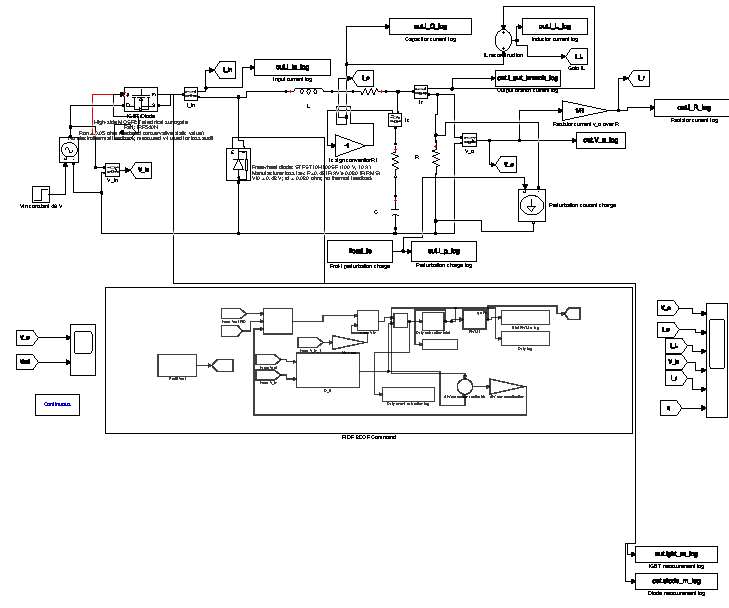
\includegraphics[width=0.82\textwidth]{figures/fig2_switched_model.pdf}
\caption{Reference Simulink/Simscape Electrical switching model (fixed \SI{48}{V} source, IRF540N surrogate, STPST10H100SF diode, resistive snubber, continuous PWM at \SI{50}{kHz}, sampled controller subsystem and energy loggers). Only the controller S-function is replaced when a candidate is replayed.}
\label{fig:slx}
\end{figure*}
